\usetikzlibrary {arrows}
\usetikzlibrary {shapes.geometric}
\usetikzlibrary {patterns}

\chapter{Background}

\section{The Semantic Web}
\hspace*{0.5cm} The Semantic Web is an extension of the World Wide Web (WWW) that allows information on it to be machine-readable. \cite{semanticweb} The concept of the Semantic Web was founded by Tim Berners-Lee, founder of the WWW, with the idea that machines can easily interpret the information available on the WWW. Tim Berners-Lee initially thought of this idea in 1999 stating "I have a dream for the Web [in which computers] become capable of analyzing all the data on the Web – the content, links, and transactions between people and computers. A 'Semantic Web'" \cite{TBLBook}. Ultimately, the semantic web aims to empower the knowledge embedded online so that it can be parsed by machines. \cite{semanticweb} 

An example of these developments can be seen by a data storage project that can be interpreted by both humans and machines- Wikidata. Wikidata is a large open knowledge base that is part of the Wikimedia family (including Wikipedia) and is connected to other datasets as well. \cite{wikidata} Data is stored in WikiData using various web data storage methods such as JSON, XML and RDF (Resource Description Framework). The latter (RDF) is described in more detail in the next section.  

Another example within the project scope is MusicBrainz. MusicBrainz also provides information that is stored using RDF. \cite{musicbrainz} In this case, MusicBrainz's focus is around music so it may be more relevant and provide more specific data for the project.  

\subsection{Resource Description Framework}
\hspace*{0.5cm} Resource Description Framework (RDF) is a method in which data can be stored, similar to how data can be stored in JSON or XML formats. However, the structure of RDF is very different. The general idea of RDF revolves around the concept of linked and connected data so RDF stores data in triples with relationships between data. This enables data stored in this format to be both machine and human-readable, allowing for the reuse and extension of data semantics. \cite{rdf} Each data store follows the structure of this sentence: 

\begin{center}
   \textit{subject predicate object}
\end{center} 

\textbf{Subject:} \\
The subject is the entity that the statement is about or refers to, which is typically a resource. A resource can be a Uniform Resource Identifier (URI- a string that identifies a name or a resource on the Internet), a physical thing or an abstract concept. 

\textbf{Predicate:} \\
The predicate describes the relationship between the subject and object (i.e. how they are related). 

\textbf{Object:} \\
The object is an entity that the statement describes with relation to the subject. This can also be blank. 

RDF uses URIs to identify the entities and relationships in a dataset, hence they provide a variety of ways to represent the data, for example, RDF graphs. RDF can be used to represent any information that can be integrated with other data representation formats such as Turtle (.TTL). In this project, we will look closer at the Turtle (.TTL) format for RDF. A .TTL file stores data in RDF format (triples) with a subject, object and relationship. This format is specifically relevant when storing RDF graphs and allowing them to be readable in a human format as well as machine-readable. \cite{TTL}

\medskip
An example of an RDF statement (in Turtle- .TTL) can be seen below:

\lstset
{
    breaklines=true,
    breakatwhitespace=true,
}
\begin{center}
\begin{lstlisting}
    <http://www.example.com/Alvin> 
    <http://www.example.com/vocab#studiesAt> 
    <http://www.example.com/KCL>
\end{lstlisting}
\end{center} 

\noindent In this example, 
\begin{itemize}
\item The subject is: \textit{"http://www.example.com/Alvin"}
\item The predicate is: \textit{"http://www.example.com/vocab#studiesAt"}
\item The object is: \textit{"http://www.example.com/KCL"}
\end{itemize}

This statement indicates that the entity \textit{"http://www.example.com/Alvin"} studies at the entity \textit{"http://www.example.com/KCL"}, according to the vocabulary defined by \\\textit{"http://www.example.com/vocab"}. However, writing all the various URI links separately is very messy and can look confusing for the human reader so we use prefixes as shown below to reduce the need to write the entire link:

\lstset
{
    breaklines=true,
    breakatwhitespace=true,
}
\begin{center}
\begin{lstlisting}
    @prefix ex: <http://www.example.com/>. 
    @prefix exVocab: <http://www.example.com/vocab#>. 

    ex:Alvin exVocab:studiesAt ex:KCL
\end{lstlisting}
\end{center} 

This example uses two abbreviations of URIs and has named the alias for these URIs to be 'ex' and 'exVocab' respectively, simplifying the statement. 

An English translation of the RDF statement is written below: 

\begin{center}
    "Alvin studies at KCL". 
\end{center}

As mentioned previously, RDFs can also be visualised in graph format with numerous (links) relationships between subjects and objects, specifying their relationships. RDFs can be used to describe ontologies, which are described in the next section.

\section{Ontology}
\hspace{0.5cm} An ontology is a conceptual framework for modelling domain knowledge. \cite{ontology} Ontologies make use of RDF's triples by have two nodes (the subject and predicate) and an edge (the relationship). They act as models in which real data can be input, so these ontologies can be used again in different contexts and shared between users. These generalised models are ideal for Knowledge Graph generation because data from different contexts can be displayed in the same way using the same ontology. 

The main components of an ontology are similar to the RDF triples we have seen but have different names. They involve:
\begin{itemize}
\item \textbf{Classes}: \\
A collection of objects or things that are related to each other in some way.

\item \textbf{Relationship}: \\
A link between a class and attribute that describe how they are related to each other. 

\item \textbf{Attributes}:\\ 
A characteristic or property that a class may have, which is described by the relationship between them.

\end{itemize}

In the context of RDF statements, a connection between two nodes will have the subject and object as the nodes and the predicate will connect them, via an edge, given the relationship specified. Below, is an example of a graphical visualisation in the context of a football team:

 \bigskip
\begin{center}
    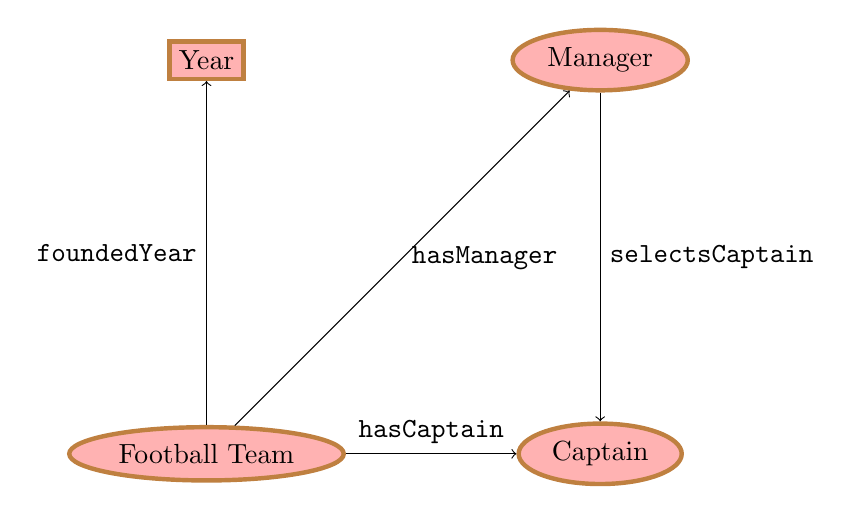
\begin{tikzpicture} [
        circle/.style={draw=brown, ellipse, ultra thick, fill=red!30},
        square/.style={draw=brown, rectangle, ultra thick, fill=red!30},
        align=center,
        node distance=5cm ]
    \node[circle] (q1)  {Football Team};
    \node[circle, right of=q1] (q2)  {Captain};
    \draw (q1) edge[->,above] node {\tt hasCaptain} (q2);
    \node[square, above of=q1] (q3) {Year};
    \draw (q1) edge[->,left] node {\tt foundedYear} (q3);
    \node[circle, above of=q2] (q3) {Manager};
    \draw (q1) edge[->,right] node {\tt hasManager} (q3);
    \draw (q3) edge[->,right] node {\tt selectsCaptain} (q2);
    \end{tikzpicture}
\end{center}

This ontology graph depicts a Football Team with a Manager and a Captain. The Manager and Captain (of the football team) also have a relationship because the manager selects a specific captain for the football team. The attribute 'Year' only describes the class 'Football Team' so is denoted as such.

Ontologies are the framework in which knowledge graphs can be constructed and guide the generation of knowledge graphs. 

\subsection{Knowledge Graphs}
\hspace{0.5cm} A knowledge graph is a graph (i.e. data graph) that depicts real-world knowledge or data. \cite{knowledgegraph} Similar to ontologies, knowledge graphs are often represented as a network of interconnected nodes and edges, but instead the nodes represent real-world entities (such as people or places) and the edges represent the real-world relationships between them (such as 'owns' or 'discovered'). 

As mentioned, knowledge graphs apply real data from an ontology graph framework. With a dataset and a relevant ontology, we can create specific instances of each ontological relationship. 

Knowledge graphs are used in a variety of real-world applications including search engines, recommendation systems and natural language processors. Common examples of these applications include:

\begin{itemize}
\item \textbf{Search Engines:} \\Knowledge graphs are used by search engines such as Google to find appropriate results given a search query. Results are interpreted and relevant information is displayed based on the relationships between the URIs and the meaning of the search term. The most relevant information with regard to the search query is displayed to the user. The method in which a knowledge graph aids a specific search query is called a "semantic search" and provides more accurate and relevant results. This mirrors how humans tend to think by emulating our natural ability to find associations between data.  \cite{searchengine}  

\item \textbf{Recommendation Systems:} \\Knowledge graphs can be in such systems because there are often many associations between different entities in a system that a recommendation program resides. Recommendation systems use relationships in the knowledge graph to display the most relevant data to the user. 

\item \textbf{Natural Language Processing:}\\ Knowledge graphs are used in this context to provide relationships between different terms that are related within the text. A system employing Natural Language Processing may want to understand the meaning of a sentence and be able to put it into a search query so that related results can be found. 

\end{itemize}

\medskip
An example of a knowledge graph can be seen below, following the ontology example displayed in the ontology section above:

\bigskip
\begin{center}
    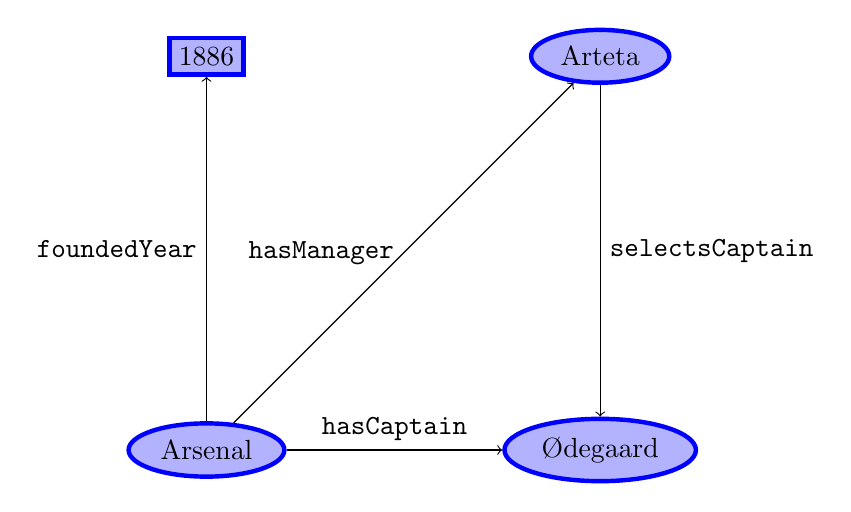
\begin{tikzpicture} [
        circle/.style={draw=blue, ellipse, ultra thick, fill=blue!30},
        square/.style={draw=blue, rectangle, ultra thick, fill=blue!30},
        align=center,
        node distance=5cm ]
    \node[circle] (q1)  {Arsenal};
    \node[circle, right of=q1] (q2)  {Ødegaard};
    \draw (q1) edge[->,above] node {\tt hasCaptain} (q2);
    \node[square, above of=q1] (q3) {1886};
    \draw (q1) edge[->,left] node {\tt foundedYear} (q3);
    \node[circle, above of=q2] (q3) {Arteta};
    \draw (q1) edge[->,left] node {\tt hasManager} (q3);
    \draw (q3) edge[->,right] node {\tt selectsCaptain} (q2);
    \end{tikzpicture}
\end{center}

The knowledge graph above describes the men's football team: Arsenal. Arteta is the manager of Arsenal and Arsenal's captain is Ødegaard. Arteta (the manager) also selects the captain. The year Arsenal was founded is depicted in the graph as 1886.

The more linked data we add from the dataset, the larger the knowledge graph will grow.

\section{SPARQL}

\hspace{0.5cm} SPARQL enables us to query RDF data formats and retrieve specific data from large RDF files. SPARQL queries often have the same structure as standard SQL queries. Specific data can be filtered by using triples by stating the subject, object and relationship format in the WHERE clause. \cite{sparlbook} An example of a SPARQL Query is shown below:

\begin{lstlisting}
PREFIX foaf: <http://xmlns.com/foaf/0.1/>
SELECT ?first_name 
       ?surname
WHERE
  {
    ?person  a          foaf:Person.
    ?person  foaf:name  ?first_name.
    ?person  foaf:surname  ?surname.
  }
\end{lstlisting}
(\textit{Example from}: \cite{foaf})

\medskip
Here the shortcut 'foaf' (friend of a friend) is used, which is often used to describe people, their characteristics, relationships and other information about them. \cite{foaf}

The SELECT part of the query wants to extract the name and surname of that person in the RDF document. 

The WHERE part of the query defines ?person of RDF type foaf:Person. That ?person has a name and a surname. 

If the query were to be executed in an appropriate RDF document, the output would list all the first names and surnames of those people who we have data about. 